
\chapter{Grundlagen} \index{Grundlagen}

TODO!!!!!!!!!

\section{LLM Tools} \index{LLM Tools} \label{LLM Tools}

Unter LLM-Tools versteht man Sprachmodelle, die auf einem Large Language Model (LLM) basieren. Ein LLM ist ein 
Deep-Learning-Algorithmus, der mit sehr großen Datensätzen trainiert wird. Diese Modelle finden häufig Anwendung im 
Bereich des Natural Language Processing (NLP), wo sie verwendet werden, um Abfragen in natürlicher Sprache zu beantworten 
oder Ergebnisse zu liefern. LLMs können neue Inhalte verstehen, zusammenfassen, generieren und vorhersagen. Durch das Training 
sammeln LLMs Milliarden von Parametern, bei denen es sich um Variablen handelt, die im Modell angepasst werden, um neue 
Inhalte abzuleiten.\\
LLMs basieren auf einem Transformer-Modell, das Eingaben in Token umwandelt und dann gleichzeitig mathematische 
Gleichungen ausführt, um Beziehungen zwischen den Token zu ermitteln. Dadurch kann der Computer Muster erkennen, 
die auch ein Mensch wahrnehmen würde, wenn ihm die gleiche Frage gestellt wird. Zudem verwenden Transformer-Modelle 
Selbstaufmerksamkeitsmechanismen, die es dem Modell ermöglichen, schneller zu lernen als herkömmliche Modelle. 
Dadurch kann das Transformer-Modell verschiedene Teile der Sequenz oder den gesamten Kontext eines Satzes berücksichtigen, 
um Vorhersagen zu generieren.

Grundsätzlich bestehen LLMs aus vier neuronalen Netzwerkschichten: der wiederkehrenden Ebene, der Einbettungsebene, 
der Feedforward-Ebene und der Aufmerksamkeitsebene. Diese Schichten arbeiten zusammen, um den Eingabetext zu verarbeiten 
und Ausgabeinhalte zu generieren.\\
Die wiederkehrende Ebene dient dazu, die Wörter des Eingabetextes der Reihe nach zu interpretieren und die Beziehungen 
zwischen den Wörtern in einem Satz zu erfassen. Die Einbettungsebene erfasst die semantische und syntaktische Bedeutung 
der Eingabe, sodass das Modell den Kontext verstehen kann. Die Feedforward-Schicht besteht aus mehreren vollständig 
verbundenen Schichten, die die Eingabeeinbettungen transformieren. Dadurch ermöglichen diese Schichten dem Modell, 
Abstraktionen auf höherer Ebene zu verstehen und somit die Absicht des Benutzers mit der Texteingabe zu erfassen. Die 
Aufmerksamkeitsebene ermöglicht es dem Sprachmodell, sich auf einzelne Teile des Eingabetextes zu konzentrieren, die für 
die Aufgabe relevant sind, und dadurch die genausten Ausgaben zu generieren.

Damit ein großes Sprachmodell Texteingaben empfangen und eine Ausgabevorhersage generieren kann, muss es zunächst 
allgemein geschult und anschließend feinabgestimmt werden, um spezifische Aufgaben ausführen zu können. Für die 
Schulung werden riesige Datenmengen im Petabyte-Bereich benötigt. Das Training verläuft mehrstufig und beginnt in 
der Regel mit einem unbeaufsichtigten Lernansatz, bei dem das Modell mit unstrukturierten und unbeschrifteten Daten 
trainiert wird, da diese in größeren Mengen verfügbar sind. In dieser Phase leitet das Modell Beziehungen zwischen 
verschiedenen Wörtern und Konzepten ab.\\
Anschließend erfolgt die Schulung und Feinabstimmung durch eine Form des selbstüberwachten Lernens. Dabei wird eine 
Datenkennzeichnung durchgeführt, durch die das Modell verschiedene Konzepte besser und genauer identifizieren kann. 
Im nächsten Schritt durchläuft das LLM den transformatorischen neuronalen Netzwerkprozess im Rahmen des Deep Learning. 
Die Transformer-Modellarchitektur ermöglicht es dem LLM, mittels eines Selbstaufmerksamkeitsmechanismus Beziehungen 
und Verbindungen zwischen Wörtern und Konzepten zu erkennen, indem bestimmten Elementen (Token) Bewertungen zugewiesen 
werden, um die Beziehungen festzulegen.

Entscheidend über die Leistungsfähigkeit und die Qualität des Sprachmodells sind die Datensätze, welche zum trainieren
benutzt werden. Im folgenden wird auf die drei unterschiedliche LLM-Tools eingeganden, welche in dieser Arbeit näher 
untersucht werden \cite{GrundlagenLLM}. 

\subsection{ChatGPT} \index{ChatGPT} \label{ChatGPT}


ChatGPT wurde von OpenAI am 30. November 2022 veröffentlicht und entwickelte sich aufgrund seiner fortschrittlichen 
generativen KI-Fähigkeiten rasch zu einer internationalen Sensation. Wenn man ChatGPT fragt, ob es einen Infotext 
zu sich selbst erstellen kann, erhält man die Antwort in \autoref{InfotextChatGPT}

\begin{figure} 
    \begin{tcolorbox}[colback=gray!20, colframe=gray!20, boxrule=0pt, sharp corners] 
    \textbf{Prompt: Erstell mir einen Infotext über dich für meine Bachelorarbeit}\\ 

    ChatGPT ist ein fortschrittlicher KI-gestützter Sprachassistent, der auf der GPT-4-Architektur von OpenAI basiert. 
    Entwickelt im Rahmen der Forschung und Entwicklung im Bereich Künstliche Intelligenz, ist ChatGPT in der Lage, 
    natürliche Sprache zu verstehen und darauf zu antworten. Dies macht ihn zu einem vielseitigen Werkzeug für eine 
    Vielzahl von Anwendungen, von der Beantwortung alltäglicher Fragen bis hin zur Unterstützung bei komplexeren 
    Aufgaben wie dem Schreiben von Texten, der Generierung von Ideen und der Bereitstellung von Informationen.\\
    
    Die GPT-4-Architektur, auf der ChatGPT basiert, verwendet tiefes maschinelles Lernen, um menschliche Sprache zu 
    verarbeiten und zu erzeugen. Durch die Analyse großer Mengen an Textdaten kann das Modell Muster und Zusammenhänge 
    erkennen, die es ihm ermöglichen, kontextuell relevante und kohärente Antworten zu geben. Diese Fähigkeiten machen 
    ChatGPT zu einem nützlichen Instrument in Bereichen wie Bildung, Forschung, Kundenservice und mehr.\\
    
    Ein weiterer bemerkenswerter Aspekt von ChatGPT ist seine Fähigkeit, sich an eine Vielzahl von Themen anzupassen 
    und Informationen auf klare und präzise Weise zu vermitteln. Dies wird durch kontinuierliches Training und 
    Verbesserung des Modells erreicht, wobei sowohl technische Fortschritte als auch Nutzerfeedback berücksichtigt 
    werden.\\
    
    Zusammengefasst ist ChatGPT ein leistungsstarker und vielseitiger KI-Assistent, der durch seine fortschrittliche 
    Technologie und seine breite Anwendbarkeit einen wertvollen Beitrag in vielen Bereichen leistet.\\
    \vfill
    \end{tcolorbox}
    \caption{Infotext ChatGPT, Quelle: ChatGPT}
    \label{InfotextChatGPT}
\end{figure}

Die Beta-Version der Plattform war zunächst kostenlos verfügbar, und OpenAI bot den Nutzern weiterhin eine kostenlose 
Basisversion an. Im Februar 2023 führte OpenAI ein kostenpflichtiges Abonnement ein, das unbegrenzten Zugriff auf ChatGPT 
sowie eine erweiterte Palette von Funktionen und Diensten ermöglichte.

Trotz der begeisterten Resonanz löste ChatGPT auch einige Kontroversen aus. Es lieferte teilweise fehlerhafte Antworten, 
insbesondere bei Aufgaben wie Schlussfolgerungen ziehen, Nuancen analysieren, Meinungen bewerten oder Vorhersagen treffen. 
Pädagogen weltweit äußerten Bedenken hinsichtlich des Einsatzes von ChatGPT im Bildungsbereich, auch an Universitäten wurde 
der Einsatz kritisch diskutiert.

Trotz dieser Kontroversen schien ChatGPT bereit zu sein, die Erstellung von Inhalten im Internet zu revolutionieren. 
Webentwickler und Content-Ersteller nutzten ChatGPT zunehmend als Recherche- und Schreibhilfe für Website-Texte.

Im März 2023 brachte OpenAI eine neue Version heraus, bekannt als GPT-4. Ein bedeutender Unterschied zu früheren Versionen 
bestand darin, dass GPT-4 Eingaben sowohl in Text- als auch in Bildformaten akzeptierte. Dies ermöglichte dem Chatbot, Daten 
aus Diagrammen, Grafiken und Screenshots zu interpretieren. Zudem machte GPT-4 deutlich weniger Denkfehler und sachliche Fehler, 
auch "Halluzinationen" genannt, als das zuvor verwendete GPT-3.5-Modell. Am Ende des Jahres hatte sich ChatGPT weiterentwickelt 
und konnte beispielsweise Bilder analysieren, Sprachansagen verarbeiten und gesprochene Antworten geben.

Im Mai 2024 kündigte OpenAI ein aktualisiertes Modell namens ChatGPT-4o an, das schnellere Ergebnisse sowie verbesserte 
Text- und Audiofunktionen versprach. Dieses Modell umfasste auch ein neues Konversations-KI-System namens ``Sky'' \cite{GrundlagenChatGPT}.

\subsection{Google Gemini} \index{Google Gemini} \label{Google Gemini}

Im Dezember 2023 stellte Google eine generative Künstliche Intelligenz mit dem Namen Google Gemini vor. Sie wurde von Google DeepMind 
entwickelt und ist laut Aussage von Google das größte, leistungsstärkste und vielseitigste große Sprachmodell (LLM), das bisher von 
Google entwickelt und realisiert wurde. In der ursprünglichen Ankündigung wurde das KI-Sprachmodell unter dem Namen Gemini vorgestellt. 
Im Februar 2024 entschied Google, auch den bisher als Bard bekannten Chatbot in Gemini umzubenennen. Damit ist Gemini mittlerweile sowohl
der Name des Google Chatbots als auch des zugrundeliegenden Sprachmodells.

Bei Nachfrage an Gemini, ob es einen Infotext über sich erstellen kann, erhält man die Antwort in \autoref{InfotextGemini1} und \autoref{InfotextGemini2}

\begin{prompt}
    \begin{tcolorbox}[colback=gray!20, colframe=gray!20, boxrule=0pt, sharp corners] 
    \textbf{Prompt: Erstell mir einen Infotext über dich für meine Bachelorarbeit}\\ 
        \textbf{Was ist Gemini?}\\
        Gemini ist ein Large Language Model (LLM) von Google AI, das mit einem riesigen Datensatz aus Text und Code 
        trainiert wurde. Es kann Text generieren, Sprachen übersetzen, verschiedene Arten von kreativen Inhalten schreiben 
        und Ihre Fragen auf informative Weise beantworten. Gemini befindet sich noch in der Entwicklung, hat aber bereits gelernt,
        viele Arten von Aufgaben auszuführen, einschließlich:
        \begin{itemize}
            \item Befolgen Sie Anweisungen und erledigen Sie Aufgaben sorgfältig.
            \item Beantworten Sie Ihre Fragen umfassend und informativ, auch wenn sie offen, herausfordernd oder seltsam sind.
            \item Generieren Sie verschiedene kreative Textformate, wie Gedichte, Codes, Skripte, Musikstücke, E-Mails, Briefe usw. 
                  Ich werde mein Bestes tun, um alle Ihre Anforderungen zu erfüllen.
        \end{itemize}
        \textbf{Technische Details}\\
        Gemini basiert auf der Transformer-Architektur und wird mit einem massiven Datensatz aus Text und Code trainiert. 
        Es verwendet eine Vielzahl von Techniken, um seine Leistung zu verbessern, einschließlich:
        \begin{itemize}
            \item \textbf{Aufmerksamkeit:} Ermöglicht es Gemini, sich auf die relevantesten Teile einer Eingabe zu konzentrieren.
            \item \textbf{Beam Search:} Ermöglicht Gemini, die besten möglichen Ausgaben zu generieren.
            \item \textbf{Multitasking:} Ermöglicht Gemini, mehrere Aufgaben gleichzeitig zu lernen und auszuführen.
        \end{itemize}
        \textbf{Anwendungen}\\
        Gemini kann für eine Vielzahl von Anwendungen eingesetzt werden, einschließlich:
        \begin{itemize}
            \item \textbf{Generierung von kreativen Inhalten:} Gemini kann verwendet werden, um Gedichte, Codes, Skripte, Musikstücke, 
            E-Mails, Briefe usw. zu generieren.
            \item \textbf{Sprachübersetzung:} Gemini kann verwendet werden, um Text von einer Sprache in eine andere zu übersetzen.
            \item \textbf{Beantwortung von Fragen:} Gemini kann verwendet werden, um Ihre Fragen umfassend und informativ zu beantworten, 
            auch wenn sie offen, herausfordernd oder seltsam sind.
            \item \textbf{Zusammenfassen von Texten:} Gemini kann verwendet werden, um lange Textpassagen zu zusammenfassen.
            \item \textbf{Schreiben verschiedener Arten von kreativen Textformaten:} Gemini kann verwendet werden, um verschiedene Arten von 
            kreativen Textformaten zu schreiben, wie Gedichte, Codes, Skripte, Musikstücke, E-Mails, Briefe usw.
        \end{itemize}
    \vfill
    \end{tcolorbox}
    \caption{Infotext Gemini 1, Quelle: Gemini}
    \label{InfotextGemini1}
\end{prompt}

\begin{figure} 
    \begin{tcolorbox}[colback=gray!20, colframe=gray!20, boxrule=0pt, sharp corners] 
        \textbf{Ethische Überlegungen}\\
        Es ist wichtig, Gemini verantwortungsvoll und ethisch zu nutzen. Zu den ethischen Überlegungen, die bei der Verwendung von Gemini zu beachten sind, gehören:
        \begin{itemize}
            \item \textbf{Vermeidung von Vorurteilen:} Gemini wird mit einem riesigen Datensatz aus Text und Code trainiert. Dieser Datensatz 
            kann Vorurteile enthalten, die sich in den Ausgaben von Gemini widerspiegeln können. Es ist wichtig, sich dieser Vorurteile bewusst 
            zu sein und Maßnahmen zu ergreifen, um sie zu mindern.
            \item \textbf{Vermeidung von Schadenszufügung:} Gemini kann verwendet werden, um schädlichen Text zu generieren, z. B. Hassreden 
            oder Gewaltandrohungen. Es ist wichtig, Gemini nicht zu verwenden, um anderen Schaden zuzufügen.
            \item \textbf{Respekt vor der Privatsphäre:} Gemini kann verwendet werden, um personenbezogene Daten zu generieren. Es ist wichtig, 
            Gemini nicht zu verwenden, um die Privatsphäre anderer zu verletzen.
        \end{itemize}
        \textbf{Fazit}\\
        Gemini ist ein leistungsstarkes Tool, das für eine Vielzahl von Anwendungen eingesetzt werden kann. Es ist jedoch wichtig, Gemini verantwortungsvoll und ethisch zu nutzen.
    \vfill
    \end{tcolorbox}
    %\addtocounter{figure}{-1}
    \caption{Infotext Gemini 2, Quelle: Gemini}
    \label{InfotextGemini2}
\end{figure}

Gemini 1.0 wurde in drei verschiedenen Größen optimiert: Gemini Ultra als das größte und leistungsstärkste Modell 
für hochkomplexe Aufgaben, Gemini Pro als das beste Modell zur Anwendung in einem breiten Aufgabenspektrum und Gemini 
Nano als das effizienteste Modell für Aufgaben, die direkt auf dem Gerät verarbeitet werden.

Die Gemini-Modelle sind von Grund auf multimodal konzipiert, was bedeutet, dass sie mit verschiedenen Arten von 
Informationen umgehen können. Gemini ist in der Lage, Texte, Programmcode, Bilder, Videos, Audioinformationen und 
deren Kombinationen zu analysieren, zu verstehen, zu kombinieren und zu generieren. Da Gemini auch mit Skizzen und 
handgeschriebenem Text umgehen kann, eignet es sich für den Einsatz in Fachbereichen wie Mathematik oder Physik und 
anderen. Im Programmierbereich werden gängige Programmiersprachen wie Python, Java, C++ oder Go unterstützt. Gemini 
kann Programmcode analysieren, kommentieren und auch generieren. Dadurch steht Gemini in Konkurrenz zu anderen LLMs 
wie den GPT-Sprachmodellen von Open AI. Gemini soll jedoch die Konkurrenzprodukte in vielen Benchmarks deutlich übertreffen.

Gemini baut auf den ebenfalls von Google entwickelten Sprachmodellen LaMDA und PaLM 2 auf. Wie üblich für 
LLMs (Large Language Models) basiert auch Gemini auf einer Transformer-Architektur. Google hat die Architektur des 
Modells zur Skalierung der Trainingsfähigkeiten optimiert und mit einem Multi-Query-Aufmerksamkeitsmechanismus ausgestattet. 
Die unterstützte Kontextlänge beträgt 32.000 Tokens und in der Version 1.5 bis zu einer Million Tokens. Gemini wurde mit 
Daten verschiedener Modalitäten trainiert, und als Trainingsplattform verwendete Google Rechner-Cluster und Tensor 
Processing Units (TPUs) der neuesten Generation v4 und v5 als KI-Beschleuniger.

Google hat begonnen, die KI in zahlreiche eigene Produkte zu integrieren, um die Fähigkeiten der Websuche, des 
Chrome-Browsers, des Gmail-Services, verschiedener Entwicklungstools und anderer Produkte und Services zu verbessern 
und zu erweitern. Mitte Februar 2024 stellte Google Gemini 1.5 und 1.5 Pro vor, welche bis zu eine Million Tokens 
verarbeiten können. Diese neuen Versionen sollen die Benchmark-Ergebnisse der Vorgängerversion deutlich übertreffen \cite{GrundlagenGemini}.

\subsection{Le Chat} \index{Le Chat} \label{Le Chat}

\begin{figure} 
    \begin{tcolorbox}[colback=gray!20, colframe=gray!20, boxrule=0pt, sharp corners] 
        \textbf{Prompt: Erstell mir einen Infotext über Le Chat für meine Bachelorarbeit}
        \textbf{Einleitung}\\
        Le Chat ist ein fortschrittliches Sprachmodell, das auf künstlicher Intelligenz (KI) und maschinellem Lernen 
        basiert. Entwickelt von einem Team aus Experten für KI und Sprachverarbeitung, hat Le Chat die Fähigkeit, 
        menschliche Sprache zu verstehen, zu interpretieren und darauf zu reagieren, was es zu einem wertvollen 
        Werkzeug in verschiedenen Branchen macht.\\

        \textbf{Funktionsweise}\\
        Le Chat nutzt eine Kombination aus Techniken des Natural Language Processing (NLP) und des Deep Learning. NLP 
        ermöglicht es dem Modell, die Struktur und den Kontext der menschlichen Sprache zu verstehen, während Deep 
        Learning-Algorithmen verwendet werden, um Muster in den Daten zu erkennen und die Genauigkeit der Vorhersagen 
        zu verbessern.\\

        \textbf{Anwendungsbereiche}\\
        Le Chat kann in einer Vielzahl von Anwendungen eingesetzt werden. Einige der wichtigsten Anwendungsbereiche sind:
        \begin{itemize}
            \item \textbf{Kundenservice:} Le Chat kann als virtueller Assistent eingesetzt werden, um Kundenanfragen zu 
            beantworten, Produktempfehlungen auszusprechen und den Kunden bei der Lösung von Problemen zu unterstützen.
            \item \textbf{Bildung:} Le Chat kann als Tutor-System eingesetzt werden, um Schülern und Studenten bei der 
            Lösung von Aufgaben und beim Verständnis von komplexen Konzepten zu helfen.
            \item \textbf{Gesundheitswesen:} Le Chat kann als virtueller Gesundheitsassistent eingesetzt werden, um 
            Patienten bei der Verwaltung ihrer Medikamente zu unterstützen, Gesundheitstipps zu geben und in Notfällen 
            Erste Hilfe-Anweisungen bereitzustellen.
            \end{itemize}
        \textbf{Vorteile}\\
        Le Chat bietet eine Reihe von Vorteilen gegenüber herkömmlichen Sprachmodellen. Einige der wichtigsten Vorteile sind:
        \begin{itemize}
            \item \textbf{Verbesserte Genauigkeit:} Le Chat nutzt fortschrittliche Deep Learning-Algorithmen, um die 
            Genauigkeit der Vorhersagen zu verbessern und eine bessere Benutzererfahrung zu bieten.
            \item \textbf{Skalierbarkeit:} Le Chat kann leicht skaliert werden, um eine große Anzahl von Anfragen 
            gleichzeitig zu bearbeiten, was es zu einer idealen Lösung für Unternehmen mit hohem Kundenaufkommen macht.
            \item \textbf{Kosteneffizienz:} Le Chat kann als kosteneffiziente Alternative zu menschlichen 
            Kundenservice-Mitarbeitern eingesetzt werden, was zu erheblichen Einsparungen für Unternehmen führen kann.
            \end{itemize}
        \textbf{Fazit}\\
        Le Chat ist ein innovatives Sprachmodell, das die Fähigkeit hat, die Art und Weise, wie wir mit Maschinen 
        interagieren, zu revolutionieren. Mit seiner fortschrittlichen Technologie und seinen vielfältigen 
        Anwendungsmöglichkeiten ist Le Chat ein wichtiger Meilenstein in der Entwicklung der KI und ein Werkzeug, 
        das in Zukunft eine noch größere Rolle spielen wird.
        \vfill
    \end{tcolorbox}
    \caption{Infotext LeChat, Quelle: Le Chat}
    \label{InfotextLeChat}
\end{figure}

In \autoref{InfotextLeChat} sieht man die Antwort die Le Chat gibt, wenn man ihn nach einem Infotext über sich 
fragt. Le Chat ist ein, von dem französischem KI-Startup Mistral AI veröffentlichter Chatbot. Mistral AI startete mit  
seinen frei verwendbaren Sprachmodellen, also auf der Grundlage von Open Source, erfolgreich durch. Nun  
hat Mistral AI sein bislang größtes Modell 'Mistral Large' veröffentlicht. Diesmal allerdings nicht auf der  
Basis von Open Source, sondern ausschließlich über die eigene Webseite und der KI-Infrastruktur Microsoft  
Azure. Es lassen sich allerdings API-Keys für Programmierschnittstellen erstellen, um z.B. Mistral Large über  
seinen eigenen Server laufen zu lassen und so für andere User auf der eigenen Homepage verfügbar zu machen.  
Mit Mistral Large wurde auch Le Chat veröffentlicht, welcher aktuell kostenfrei verwendet werden kann.
Le Chat bietet derzeit noch sehr wenige Funktionen an. Es stehen Lediglich Texteingabe und -ausgabe zur Verfügung.  
Die Datengrundlage reicht nur bis 2021, weshalb es auch hier, für die Jahre 2022 bis heute, zu der Problematik der  
Halluzination kommen kann.
Grundsätzlich kann man zwischen drei Sprachmodellen auswählen: Large, Next und Small. Large bietet überlegene Denkfähigkeit,  
Next ist ein Prototyp-Modell für erhöhte Kürze und Small arbeitet schnell und kosteneffektiv \cite{GrundlagenLeChat}.


\section{Software Engineering Prozess}

\begin{figure}
    \centering
    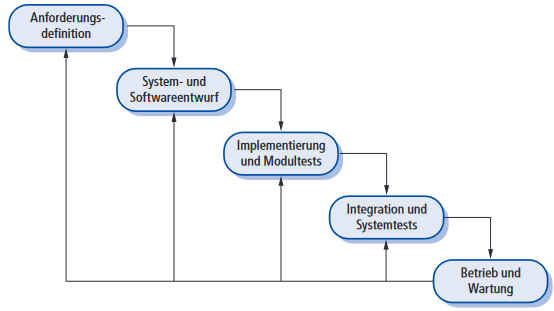
\includegraphics{pictures/Wasserfallmodell.PNG}
    \caption{Wasserfallmodell, Quelle: \cite{Sommerville10}}
    \label{Ablauf Wasserfallmodell}
\end{figure}

Software-Engineering ist eine technische Disziplin, die sich umfassend mit der Erstellung von Software beschäftigt, beginnend 
bei der Konzeption, über den Betrieb, bis hin zur Wartung. Die wesentlichen Aktivitäten im Software-Engineering umfassen die 
Softwarespezifikation, -entwicklung, -validierung und -weiterentwicklung. Die Arbeitsweise im Software-Engineering variiert 
je nach den spezifischen Umständen. Für bestimmte Softwaretypen kann daher ein kreativeres, weniger formelles Vorgehen angemessen 
sein. Im Mittelpunkt des Software-Engineerings steht somit die Auswahl der am besten geeigneten Methode. Dieser systematische 
Ansatz wird oft als Softwareprozess bezeichnet. Ein Softwareprozess besteht aus einer Abfolge von Aktivitäten, die zur Erstellung 
eines Softwareprodukts führen. Die vier grundlegenden Aktivitäten des Software-Engineerings sind in jedem Softwareprozess 
enthalten. In dieser Arbeit wird ausschließlich das Wasserfallmodell als Softwareprozess behandelt. Das Wasserfallmodell ist das 
erste veröffentlichte Modell für die Softwareentwicklung und basiert auf Prozessmodellen, die ursprünglich in der Entwicklung 
großer militärischer Systeme verwendet wurden. Das Modell stellt den Softwareentwicklungsprozess als eine Reihe von Phasen dar, 
wie in \autoref{Ablauf Wasserfallmodell} veranschaulicht. Das Wasserfallmodell ist ein Beispiel für einen plangesteuerten Prozess, 
bei dem alle Prozessaktivitäten inhaltlich und zeitlich geplant werden, bevor die eigentliche Softwareentwicklung beginnt. Im 
Folgenden werden die einzelnen Phasen des Wasserfallmodells beschrieben \cite{Sommerville10}.

\subsection{Anforderungsdefinition} \index{Anforderungsdefinition} \label{Anforderungsdefinition}

Die erste Phase des Wasserfallmodells umfasst die Analyse und Definition der Anforderungen. Dabei werden in Zusammenarbeit mit den 
Systembenutzern die Dienstleistungen, Einschränkungen und Ziele des Systems ermittelt. Diese Anforderungen werden anschließend 
detailliert spezifiziert und dienen als Grundlage für die Systemspezifikation \cite{Sommerville10}. Die Ergebnisse dieser Phase werden in einem Dokument, 
der Anforderungsspezifikation, festgehalten.\\

Die Anforderungsspezifikation umfasst die Benutzeranforderungen, eine grobe Systemübersicht mit der benötigten Hardware, sowie ein 
fachliches Datenmodell, das die erforderlichen Klassen, deren Variablen und Beziehungen beschreibt. Zudem enthält sie ein 
Anwendungsfalldiagramm, das die gewünschten Anwendungsfälle den entsprechenden Rollen zuweist, und eine detaillierte Beschreibung 
jedes Anwendungsfalls, einschließlich eines Entitätendiagramms zur Festlegung des Ablaufs. Des Weiteren beinhaltet die Spezifikation 
eine Skizzierung und Beschreibung der erforderlichen Dialoge sowie eine Benutzungsschnittstelle, die die verschiedenen Dialoge 
miteinander verknüpft. Abschließend werden die nichtfunktionalen Anforderungen zusammen mit einem entsprechenden Test festgehalten.\\

Diese umfassende Dokumentation bildet die Basis für die nachfolgenden Phasen im Wasserfallmodell und stellt sicher, dass alle 
Anforderungen klar und präzise definiert sind.

\subsection{System- und Softwareentwurf} \index{System- und Softwareentwurf} \label{System- und Softwareentwurf}

Die zweite Phase des Wasserfallmodells ist der System- und Softwareentwurf. Im Rahmen des Systementwurfsprozesses werden die Anforderungen 
entweder Hard- oder Softwaresystemen zugewiesen, wodurch eine übergeordnete Systemarchitektur festgelegt wird. Der Softwareentwurf konzentriert 
sich auf das Erkennen und Beschreiben der grundlegenden abstrakten Softwaresysteme und ihrer Beziehungen zueinander \cite{Sommerville10}. Die 
Ergebnisse dieser Phase werden in einem Architekturdokument festgehalten.\\

Das Architekturdokument umfasst eine Skizze und eine Beschreibung der technischen Infrastruktur, die eine ausführlichere Version der Systemübersicht 
aus der Anforderungsspezifikation darstellt [\ref{Anforderungsdefinition}]. Zudem beinhaltet es ein Komponentenmodell, in dem die Schnittstellen zwischen den einzelnen 
benötigten Komponenten dargestellt und beschrieben werden. Weiterhin enthält das Architekturdokument eine detaillierte Schnittstellenbeschreibung, 
in der die Schnittstellen der Komponenten für die Implementierung festgelegt werden. Abschließend wird für jeden Anwendungsfall ein Sequenzdiagramm 
erstellt, das festlegt, welche Funktionen in den jeweiligen Schnittstellen der Komponenten vorhanden sein müssen.\\

Diese detaillierte Dokumentation ist essenziell, um sicherzustellen, dass die Softwareentwicklung auf einer klaren und präzisen Architektur 
basiert, die alle Anforderungen berücksichtigt und eine effiziente Implementierung ermöglicht.

\subsection{Implementierung und Modultests} \index{Implementierung und Modultests} \label{Implementierung und Modultests}

Die Implementierung und die dazugehörigen Modultests finden in der dritten Phase des Wasserfallmodells statt. In dieser Phase wird der 
Softwareentwurf durch eine Reihe von Programmen oder Programmeinheiten realisiert. Die Modultests stellen sicher, dass jede Einheit ihre 
Spezifikation erfüllt \cite{Sommerville10}. Je mehr Tests erstellt werden, desto besser kann die Funktionalität der Implementierung gewährleistet 
werden. Daher sollten möglichst viele Tests durchgeführt werden. Diese Tests konzentrieren sich auf die einzelnen Komponenten. Wenn eine Komponente von 
einer anderen abhängig ist, kann zunächst mit einem Dummy getestet werden. Bei der Zusammenführung der einzelnen Komponenten wird dann nochmals mit der 
echten Komponente getestet [\ref{Integration und Systemtests}]. Ein Dummy dient dabei als Ersatz für ein (noch) nicht vorhandenes Unterprogramm, in dem die gewünschte Ausgabe simuliert wird. 
In dieser Phase werden die Tests in der Testspezifikation dokumentiert.\\

Die Testspezifikation umfasst ein Testkonzept, das festlegt, wann welche Komponente getestet wird und ob bei Abhängigkeiten von anderen Komponenten auf 
die fertige Implementierung gewartet oder zunächst ein Dummy verwendet wird. Für die Modultests werden für jeden Anwendungsfall Tests erstellt, die mit einer 
Vorbedingung, einem bestimmten Testablauf und dem erwarteten Ergebnis beschrieben werden. Dazu gehört auch eine Tabelle mit den Testdaten, die die Tester 
verwenden sollen. Außerdem gibt es ein Testprotokoll, in dem die Ergebnisse der Tests festgehalten werden.\\

Diese detaillierte Dokumentation der Tests ist entscheidend, um sicherzustellen, dass jede Programm- oder Programmeinheit korrekt funktioniert und den 
festgelegten Spezifikationen entspricht.

\subsection{Integration und Systemtests} \index{Integration und Systemtests} \label{Integration und Systemtests}

Die vierte Phase des Wasserfallmodells befasst sich mit der Integration und den Systemtests. In dieser Phase werden die einzelnen Programmeinheiten oder 
Programme zusammengeführt und als Gesamtsystem getestet, um sicherzustellen, dass die Softwareanforderungen erfüllt werden. Nach Abschluss der Tests wird 
das Softwaresystem an den Kunden ausgeliefert \cite{Sommerville10}.\\

Die Systemtests werden nach dem gleichen Verfahren erstellt wie die Modultests in der dritten Phase [\ref{Implementierung und Modultests}] und sind ebenfalls 
in der Testspezifikation dokumentiert. Diese Tests dienen dazu, die Funktionsweise des gesamten Systems zu überprüfen und sicherzustellen, dass alle 
Komponenten korrekt zusammenarbeiten und die festgelegten Anforderungen erfüllen.

\subsection{Betrieb und Wartung} \index{Betrieb und Wartung} \label{Betrieb und Wartung}

Die letzte, fünfte Phase des Wasserfallmodells umfasst den Betrieb und die Wartung. Diese Phase ist normalerweise die längste im gesamten Lebenszyklus 
der Software. In dieser Phase wird das System installiert und für den Gebrauch freigegeben. Die Wartung beinhaltet das Korrigieren von Fehlern, die in
den vorherigen Phasen nicht entdeckt wurden, die Optimierung der Implementierung von Systemeinheiten und die Anpassung des Systems an neue Anforderungen, 
die nach der Freigabe auftreten \cite{Sommerville10}.